% ============================================================================ %
% =                                                                          = %
% = project-manifest.tex                                                     = %
% = This LaTeX file generates the project proposal document, which is        = %
% = distributed publicly and used to represent the project to interested     = %
% = interested parties.                                                      = %
% =                                                                          = %
% ============================================================================ %

\documentclass[12pt,draft,oneside]{article}
\usepackage{times,caption,listings,color,url,datetime,ifthen}
\usepackage{subcaption,multicol,nameref}
\usepackage[margin=1in]{geometry}
\usepackage[pdftex]{graphicx}
\usepackage[bookmarks]{hyperref}

% Uncomment These When Rendering as Draft
\usepackage{draftwatermark}
%\usepackage{showframe}

% Apply Styling Options
\linespread{1.20}
\usepackage[default]{opensans}
\usepackage[T1]{fontenc}
\usepackage{enumitem}
\setlist{noitemsep}
\usepackage[compact]{titlesec}
\titlespacing*{\section} {0pt}{30pt}{20pt}
\titlespacing*{\subsection} {0pt}{3.5ex plus 1ex minus .2ex}{2.3ex plus .2ex}
\renewcommand{\abstractname}{\null}
\renewcommand{\contentsname}{Contents}
\renewcommand{\listfigurename}{Figures}
\renewcommand{\refname}{\null}

% Use a Custom Header
\usepackage{fancyhdr,lastpage}
%\let\oldtitle\title             \renewcommand{\title}[1]{\oldtitle{#1}\def\titletext{#1}}
%\let\oldchaptermark\sectionmark \renewcommand{\sectionmark}[1]{\markboth{\thechapter.\ #1}{}}
\pagestyle{fancy}{
  \fancyhead{} % clear all fields
  \lhead{\leftmark}
  \rhead{pg.~\thepage}
  \lfoot{} \rfoot{}
  \chead{} \cfoot{}
}


\title{Small Parts Vending Machine\\ Project Status Report}
\author{Embedded Hardware Club\\ Rensselaer Polytechnic Institute}
\date{November 2012}


\begin{document}


\maketitle
\thispagestyle{empty}
\begin{abstract}
  \noindent
  Buying components from the \emph{small~parts vending~machine} is more convenient and less expensive than buying from a retailer or shipping from a catalog. The user interface is easy to use and resistant to exploitation. The location hosting the systems has the opportunity to make a fair profit.
  \\~\\
  \small
  Members of \emph{Embedded Hardware Club} can use the vending machine in the workshop to purchase small quantities of common components, including SMD and DIP chips. Users scan their RPI ID card to credit their purchase to a tab, which is charged to their bursar account at the end of each semester.
  \\~\\
  As of November 2012, the project specifications include the core machine and one type of component dispenser, the software is feature-complete, and a device prototype implements the core functionality of the specification. With additional funding, at least one complete machine can be built and further evaluated.
\end{abstract}
\pagebreak


\thispagestyle{empty}
\tableofcontents
\vfill
%\section*{Document Revision History}
%\begin{table}[b]
%  \begin{tabular}{r | l l}
%    \hline
%    Rev.          & Release     & Details       \\
%    \hline
%    A             & 2012 DEC 03 & Draft release \\
%    \hline
%  \end{tabular}
%\end{table}
\pagebreak


\section{Introduction}
\label{sec:intro}

It's the night before your project is due, and you need a \textsc{74241} octal inverter chip. And you need it now. This type of small component costs just fifty-cents, but shipping it from a traditional parts catalog can take a week and five dollars. Meanwhile, the retail stores in your neighborhood charge twice the price. You need that small component now and you deserve to pay a fair price! There is a solution--the EHC Small Parts Vending Machine is designed to consider safety, performance, and user satisfaction.

The Small Parts Vending Machine was conceived by the RPI Embedded Hardware Club in response to their own members' needs. It is a unique implementation and presents the opportunity for the host location to make a fair profit. The design is enhanced by the application of the three human factors--safety, performance, and user satisfaction--with special attention before and during the development of each subsystem.


\section{Project Information}
\label{sec:info}

\subsection{About RPI Embedded Hardware Club}
\emph{Embedded Hardware Club} is a group of students at Rensselaer Polytechnic Institute who share a passion for microcontrollers, electronics, and programming. EHC was founded in Spring 2011 as a 501(c)(3) organization funded by the Rensselaer Union. Since Spring 2012, EHC has operated jointly with the Cognitive Robotics lab in Sage 2202. Previous club projects include the ``Charliecube'' low-cost color LED cube and the RPI-RFID wireless tag reader. Current club projects include a light UAV and ``ALFRED the Butler Bot,'' an autonomous hospitality robot. %Additional details can be found at \href{http://rpiEHC.org}{rpiEHC.org}.

\subsection{Collaboration with \emph{Human Factors in Design}}
Included among the EHC team members are students in Prof. Ruecker's Fall 2012 course, \emph{Human Factors in Design} (\textsc{psyc-2220}). The four HF team members worked with EHC to complete a draft specification, functional prototype, and human factors analysis for presentation to the course in November 2012. This project was a component of the \emph{Human Factors} students' final grades, although the extent of the project and the involvement of EHC was not required by the course.

\subsection{Team Members}
Members labeled as part of the Human Factors team had specific responsibilities for the Fall 2012 semester which were evaluated for a class grade. In general, the HF and EHC teams are comprised of the same people. All team members meet in weekly meetings. Contributing team members are listed below in alphabetical order. Contact Project Lead \href{mailto:pakt@rpi.edu}{Theo Pak} for more information.

\begin{multicols}{2}
  \begin{itemize}[label=\null,labelwidth=0pt,leftmargin=0pt]
    \setlength{\itemsep}{6pt}
    \item %\textbf{Electrical System Specialist}\\
      \textbf{David Herbert} \textsc{ehc}\\
      Electrical Engineering, Class of 2013\\ herbed@rpi.edu
    \item %\textbf{Mechanical System Specialist}\\
      \textbf{James T. Kalfas} \textsc{ehc}\\
      Mechanical Engineering, Class of 2013\\ kalfajt@rpi.edu
    \item %\textbf{Mechanical and Electrical}\\
      \textbf{Anthony Kouttron} \textsc{ehc}\\
      Electrical Engineering, Class of 2014\\ koutta@rpi.edu
    \item %\textbf{Project Lead}, HF Team\\
      \textbf{Theodore X. Pak} \textsc{hf, ehc}\\
      CSYS/CSCI, Class of 2015\\pakt@rpi.edu
    \item %\textbf{Human Factors Specialist}, HF Team\\
      \textbf{James Pressly} \textsc{hf}\\
      Materials Science, Class of 2013\\ pressj2@rpi.edu
    \item %\textbf{Design Specialist}, HF Team\\
      \textbf{Caroline M. Sullivan} \textsc{hf, ehc}\\
      Undeclared Engineering, Class of 2016\\ sullic7@rpi.edu
    \item %\textbf{UI Specialist}, HF Team\\
      \textbf{Zachary E. Torre} \textsc{hf, ehc}\\
      Cognitive Science, Class of 2013\\ torrez@rpi.edu
    \item %\textbf{Mechanical Design}\\
      \textbf{Jordan Yamada} \textsc{ehc}\\
      Electrical Engineering, Class of 2016\\ yamadaj@rpi.edu
  \end{itemize}
\end{multicols}


\section{Design Specification}
\label{sec:spec}

\subsection{List of Subsystems}
\begin{enumerate}
  \item \textbf{Subsystem - Systems Management}
    \begin{enumerate}
      \item \textbf{Power Source:} AC via off-the-shelf ATX power supply
      \item \textbf{Platform:} Raspberry Pi Microcomputer - BCM2835 (ARM11)
      \item \textbf{Software:} \emph{Raspbian} Linux, Python2, pygtk, pyserial, RPi.GPIO
    \end{enumerate}
  \item \textbf{Subsystem - User Interface}
    \begin{enumerate}
      \item \textbf{Display:} VGA LCD
      \item \textbf{Interface:} Resistive Touchscreen
      \item \textbf{Payment Method:} RFID Reader via the \emph{EHC-RFID} Project
    \end{enumerate}
  \item \textbf{Subsystem - Chassis}
    \begin{enumerate}
      \item \textbf{Structural Materials:} pine lumber, plywood, steel angle brackets
      \item \textbf{Fastenings:} 1/4'' steel bolts, hex nuts, wing nuts, carpenter screws
      \item \textbf{Furnishings:} 1/8'' clear acrylic, 1/8'' clear polycarbonate
    \end{enumerate}
  \item \textbf{Subsystem - SMD Dispenser}
    \begin{enumerate}
      \item TBD
    \end{enumerate}
  \item \textbf{Subsystem - DIP Dispenser} (TBD)
  \item \textbf{Subsystem - Loose Items Dispenser} (TBD)
\end{enumerate}

\begin{figure}
  \centering
  \begin{subfigure}[b]{0.5\textwidth}
    \centering
    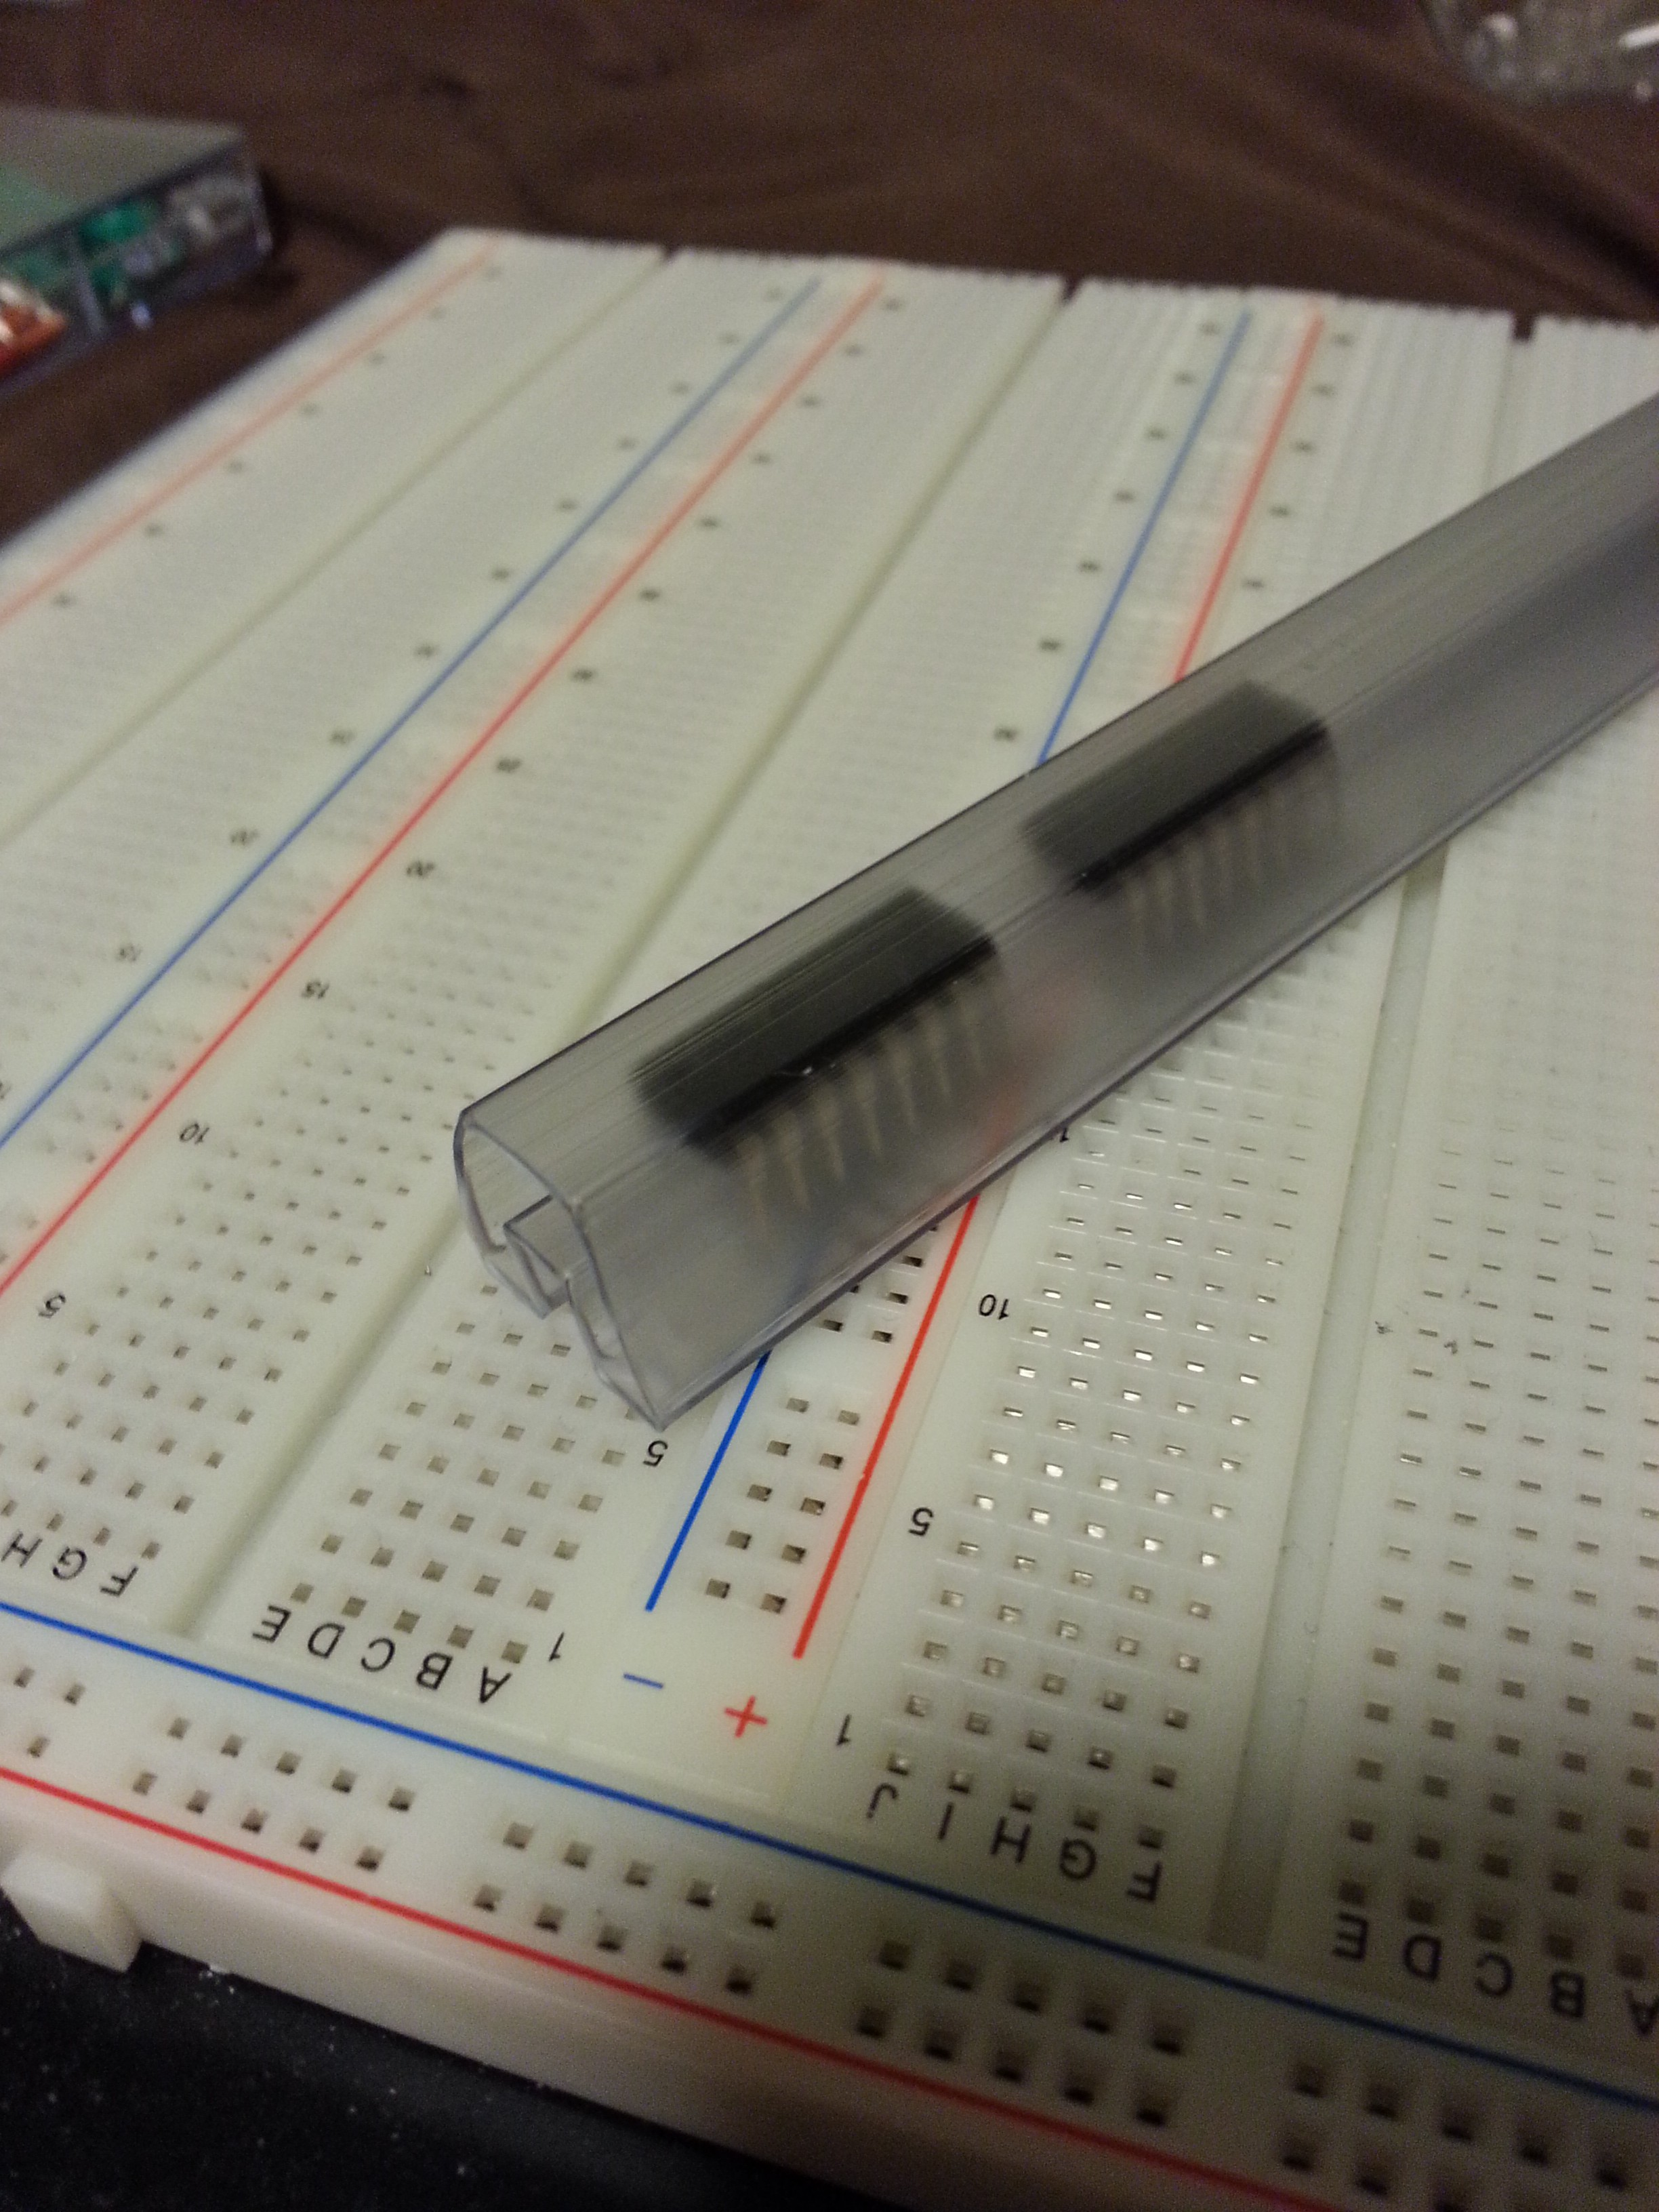
\includegraphics[width=\textwidth]{2012-09-11_dip-stick-tube.jpg}
    \caption{A plastic ``stick'' container of DIP chips}
  \end{subfigure}%
  \begin{subfigure}[b]{0.5\textwidth}
    \centering
    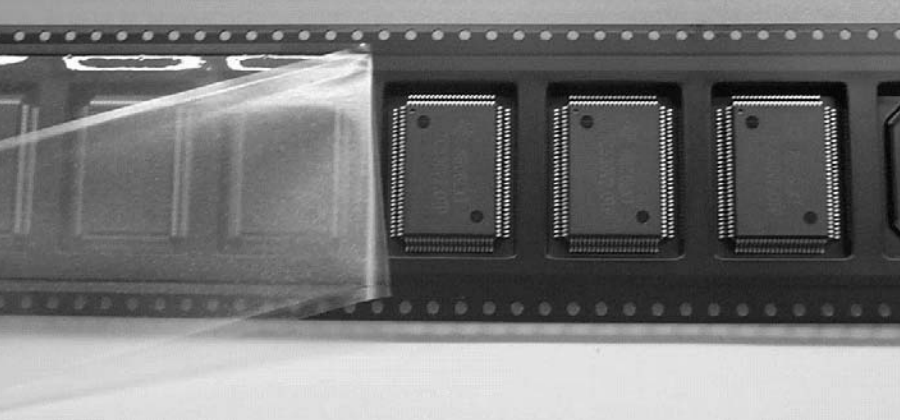
\includegraphics[width=\textwidth]{2012-12-03_smd-tape.png}
    \caption{SMD chips in an embossed carrier tape with the cover tape peeled back}
  \end{subfigure}%
  \caption{Two types of IC packages}
  \label{fig:packages}
\end{figure}

\subsection{Software Design Hierarchy}
Theo: todo

\begin{figure}
  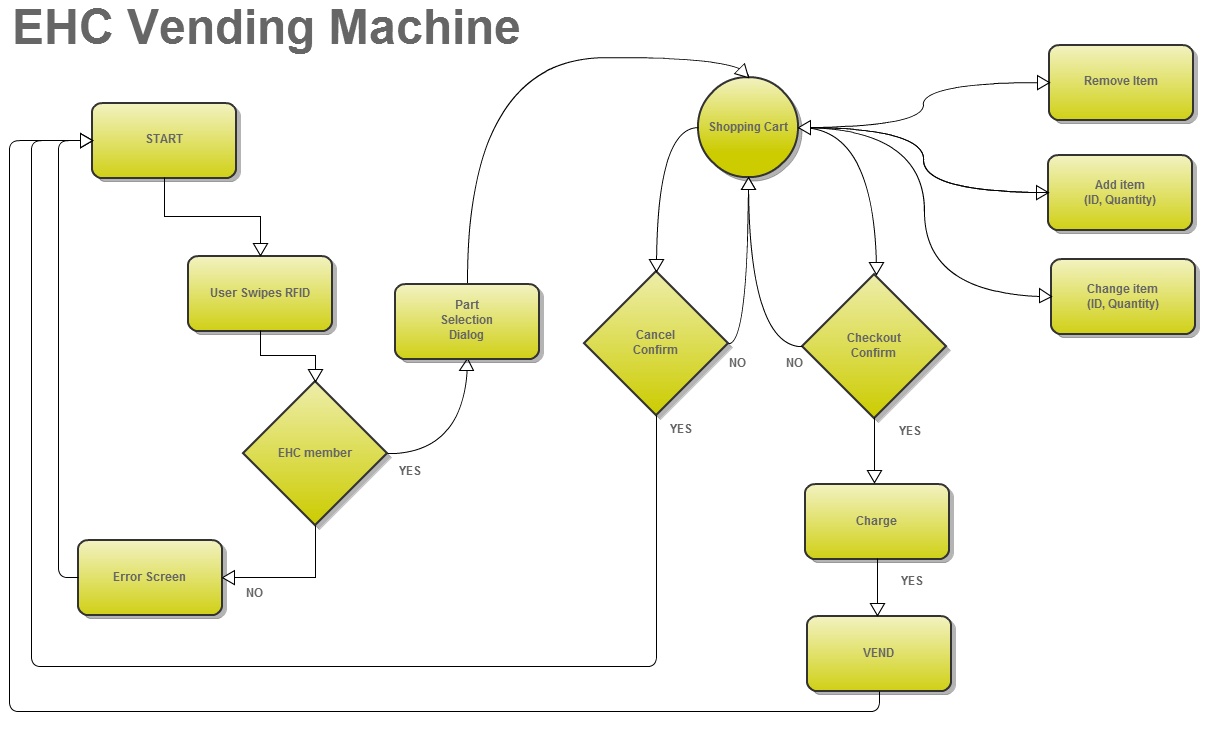
\includegraphics[width=6.5in]{2012-11-11_flowchart-of-purchase-path.png}
  \label{fig:purchase-path}
  \caption{Flowchart of Purchase Path from User Perspective}
\end{figure}


\section{Summary of Human Factors in Design}
\label{sec:hf}

\subsection{Relevant Usage and Physical Description}
The chassis was designed using an existing international standard so that mounting and removing individual units is safe, inexpensive, and modular. Each self-contained unit houses an individual component dispenser and is sized according to the Electronic Industries Association standard \textsc{eia-310}~\cite{eia-310}, which is a recent standardization of the 19-inch rack system used to mount every kind of hardware from enterprise computing to audio equipment since it was first used to house railroad signal relays. A rack unit, abbreviated ``U,'' can be up to 17-inches wide and includes 1-inch mounting brackets on each side. Units that are increments of 1.75-inches tall are said to be size U, size 2U, size 3U, and so on. This standard was adopted in favor of the competing Western Electric 23-inch-rack standard because the 19-inch-rack width is more commonly available to EHC. Prototypes were designed using free and salvaged equipment.

Users order parts from the machine by interacting with a large, color touchscreen on its face. The design process considered a number of interface options and concluded that a color display was the best way to convey information and that a large touchscreen was the most natural interaction method. This is especially true with regards to a user's prior knowledge as considered by a top-down processing model. This interface to the control unit, a Raspberry Pi micro-computer, then commands the dispensers with digital signals. The typical dispenser shelf contains a reel of stock to dispense, rollers and gears to advance the tape, a cutting mechanism to cut the tape, a tray into which the part is dispensed, and an LED light to indicate when the part is vended. Shelves are mounted in vertical stacks and such that the display elements are visually clustered in a consistent way.

\subsection{Safety}
Safety to the user and the operator was considered during design of the physical and computational subsystems so that the machine is as comfortable to use as it is functional and profitable. First, the chassis design makes provisions to bolt or weight the base so that it cannot be tipped and moved. The vending machine is also fully locked and enclosed so that none of the exposed elements are dangerous to the user. Internal components are similarly arranged so that a knowledgeable operator is shielded from cutting mechanisms and fine gearing. Second, the CIA principles of information security were applied so that personal information is protected: identity confidentiality is established by the use of an arbitrary number in place of the user's secret Rensselaer Identification Number and by an automatic time-out after inactivity; stock and transaction integrity is ensured by the physical protection of the data storage card and by the lack of network connectivity; yet accessibility is not compromised because only an instant RFID scan and confirmation of intent are required to use the machine.

\subsection{Performance}
Performance was the second human factor considered--because in order for the vending machine to be functional, it must also be simple to setup, easy to maintain, and straightforward to use. Setup is simple because of the modular design involving self-contained dispenser shelves. The operator can simply add another shelf as space allows. It is also easy for the operator to stock components when they are sold and shipped in a reel of antistatic tape, according to the latest version of the industry standard \textsc{eia-481}~\cite{eia-481}. To replace or restock a given component the operator simply slides out the dispenser, removes the old reel, inserts a new reel, and feeds the tape into the rollers. Dispensers have few points of failure because their only moving parts are few gears, rollers, and the cutting mechanism which are locked to the position of the \textsc{eia-481} carrier tape. But, over many uses, if a failure does occur then the dispenser easily slides out of the chassis for repair. Use of the vending machine is also easy thanks to the intuitive touchscreen interface. This interface translates a user's intent into software directives and digital logic signals so that the selection, transaction, and dispensing processes are managed from a single path.

\subsection{User Satisfaction}
Finally, human factors is concerned with user satisfaction while using the device. The vending machine designed for the embedded hardware club is both ergonomic and has an easy to use purchasing interface. The dispensers in the vending machine are designed to stack vertically rather than horizontally. Initially, a horizontal layout was considered so that the machine could vend components across a table and into a single drop tray. This is similar to an industrial pick-and-place automated assembly device. However, the design team realized that such a design offers this minor convenience only by sacrificing ease-of-use to the user and floor space in the host location. It was therefore decided that a vertical layout is required. The team also decided it would be easier for the user to find the components by dispensing each unique part into an individual tray, rather than one large tray, and including an LED indicator light above each tray. Walking away from the screen to view and retrieve items, as would occur in the horizontal layout, was deemed suboptimal so the vertical layout, which allows the user to stay in front of the screen while retrieving items, was pursued for the final design. The team also decided not to place dispensers low on the rack as this would make the user need to bend down to retrieve some items. The trade-off associated with this is that more racks will be needed to house the same number of dispensers but this is an acceptable trade off to ensure user satisfaction.

The screen height is another important factor of the design to consider. If the screen is too high or too low then the user will have trouble making a purchase. The average height of an American male is about 5'10'' and about 5'4'' for an American female. The team decided that the screen should be centered at a height of approximately 4'6'' or ``chest height'' for the average American male and a little below eye level for American females. To aid taller users in operating the device the screen will be angled backward slightly. This will allow taller users to view the screen more easily while still allowing shorter users to easily make a purchase.

The Graphical User Interface, or ``GUI'' was also designed to increase user satisfaction. The interface uses large touchscreen buttons to allow for easier human-computer interaction. The colors are simple and high in contrast and were chosen based on information strategies like ``top-down'' processing. For example, the ``forward'' or ``proceed'' buttons are green while the ``quit'' and ``back'' buttons remain red--the user doesn't even need to read the labels to know what these buttons do. Top down processing is also evident when the Item is out of stock. For example, when an item is out of stock, the previously blue highlight changes to red. Immediately giving the user the notion that the item may no longer available even before he or she reads the ``out of stock'' label. The buttons and labels are consistent throughout the interface, and each process in buying a part is displayed in its own window. Reinforcing a sequential process and increasing intuitiveness.

\subsection{Conclusion}
Application of human factors before and during the design process allowed planners to predict user interaction, resulting is a better design and implementation. Members of RPI Embedded Hardware Club will be able to use the vending machine in the workshop to purchase small quantities of common components like SMD and DIP chips. Users scan their RPI ID cards to credit their purchase to a tab, which is charged to their bursar account at the end of each semester. For small quantities, the vending machine is more convenient and less expensive than ordering and shipping from a catalog. The user interface is easy to use and resistant to exploitation.


\section{Remaining Challenges}
\label{sec:challenges}

\subsection{Design Specification Must Be Expanded}
As of December 2012 the \nameref{sec:spec} (see pg.~\ref{sec:spec}) defines the core system, user interface, chassis, and SMD dispenser. The other two dispenser types (DIP and loose-component dispensers) must still be designed. This requires additional mechanical design and a small extension of the device controller software.

\subsection{Machine Prototype is Inadequate for Continued Use}
The prototype machine that was demonstrated to Prof. Ruecker's class on Thursday 29 November 2012 fully implements the core system and the feature-complete user interface. The demo chassis is the width described by the design specification, but is just one-third of the height and was constructed with salvaged lumber and cardboard rather than steel and plywood, as the specification states. Additionally, time and availability constraints caused the team to miss the deadline for the SMD dispenser so that it was not functional during the 29 NOV demonstration.

Non-structural damage was caused to the cardboard and paper panels when the prototype was returned to the EHC workshop. These cosmetic damages impact the viability of the prototype as a demonstration tool, although they do not affect the functionality. Furthermore, the touchscreen used in the prototype belongs to EHC and should not be permanently mounted in a way that damages its housing.

\subsection{External Funding is Needed}
Use of EHC resources and workspace requires the approval of a club officer, however, all project budgets must conform to the club budget approved by the Rensselaer Union. External funding is required to continue work on this project because the \nameref{sec:spec} exceeds the remaining budget allotted to club projects.

\subsection{Recommendations}
Using knowledge gained while constructing and demonstrating the machine prototype, the project team prepared several recommendations to be applied when project work resumes in the Spring 2013 semester. Note that Because the

It is recommended that the final Chassis and Interface subsystems be built to the full \nameref{sec:spec} and installed in a testing environment. A locked workspace in the EHC workshop is available through the Spring 2013 semester and is well-suited as a test environment.

\appendix

\section{Gantt Chart}
\label{ref:gantt}
Theo: todo

\section{References}
\label{ref:refs}

\bibliographystyle{unsrt}
\bibliography{bibfile}
\begin{thebibliography}{1}

  % NOTE: The organization 'EIA' was known as the Electronic Industries Association prior to 1997 and as the Electronic Industries Alliance from 1997 until 2011. In 2011 the EIA was disbanded and it's working groups reorganized. Many of the standards applicable to this project fall under the Electronic Components Industries Association. But even through organizational changes and document revisions, everyone know what ANSI/EIA-310 means.

  \bibitem{eia-481} Electronic Components Industries Association, ``Taping of Surface-Mount Components for Automatic Placement,'' ANSI/EIA-481-E, Sept. 22, 2011.

  \bibitem{eia-310} Electronic Industries Association, ``Racks, Panels, and Associated Equipment,'' ANSI/EIA-310-D, 1992.

  \bibitem{rpi_vend} RPI Embedded Hardware Club, ``Small Parts Vending Machine Project Source Code,'' github.com. [Online]. Available: \url{https://github.com/rpiEHC/rpi_vend}. [Accessed Dec. 3, 2012].

\end{thebibliography}



\end{document}
